\input ../SlidePreamble
\input ../preamble


\begin{document}

{\Huge

  \centerline{\bf TTIC 31230, Fundamentals of Deep Learning}
  \bigskip
  \centerline{David McAllester, Autumn 2023}
  \vfill
  \vfil
  \centerline{Diffusion Model Guidance}
  \vfill
  \vfill

\slide{Conditional Diffusion Models and Guidance}

\centerline{Deep unsupervised learning using nonequilibrium thermodynamics}
\centerline{Sohl-Dickstein et al., 2015.}

\vfill
\centerline{Denoising Diffusion Probabilistic Models (DDPM)}
\centerline{Ho, Jain and Abbeel, (Berkeley, May 2021)}


\vfill
\centerline{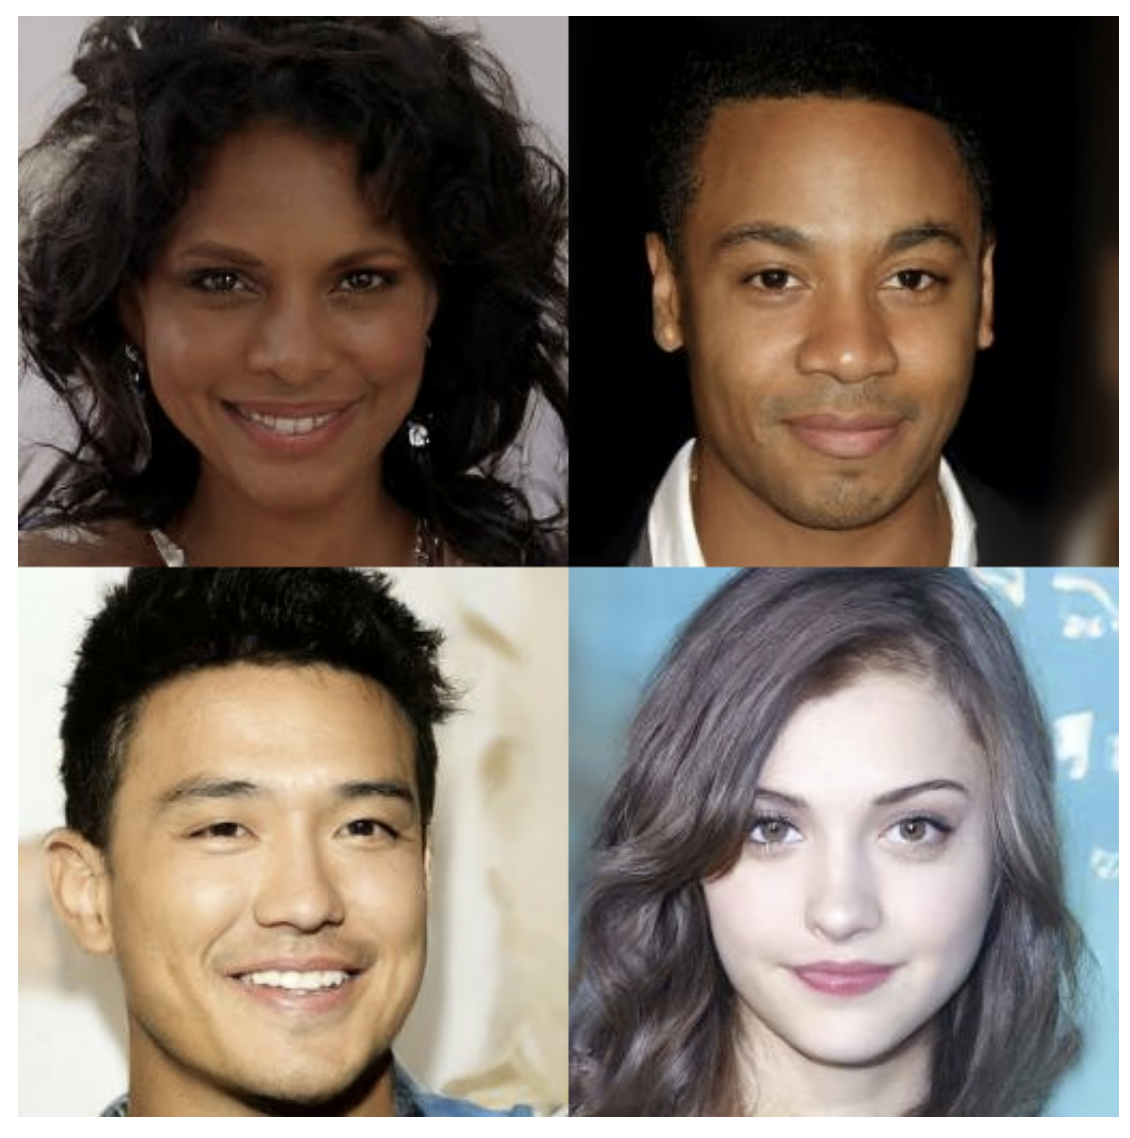
\includegraphics[width = 2.5in]{\images/DiffCeleb}}

\slidetwo{Diffusion Models Beat GANs on Image Synthesis}{Dharwali and Nichol (OpenAI, May 2021)}

\vfill
\centerline{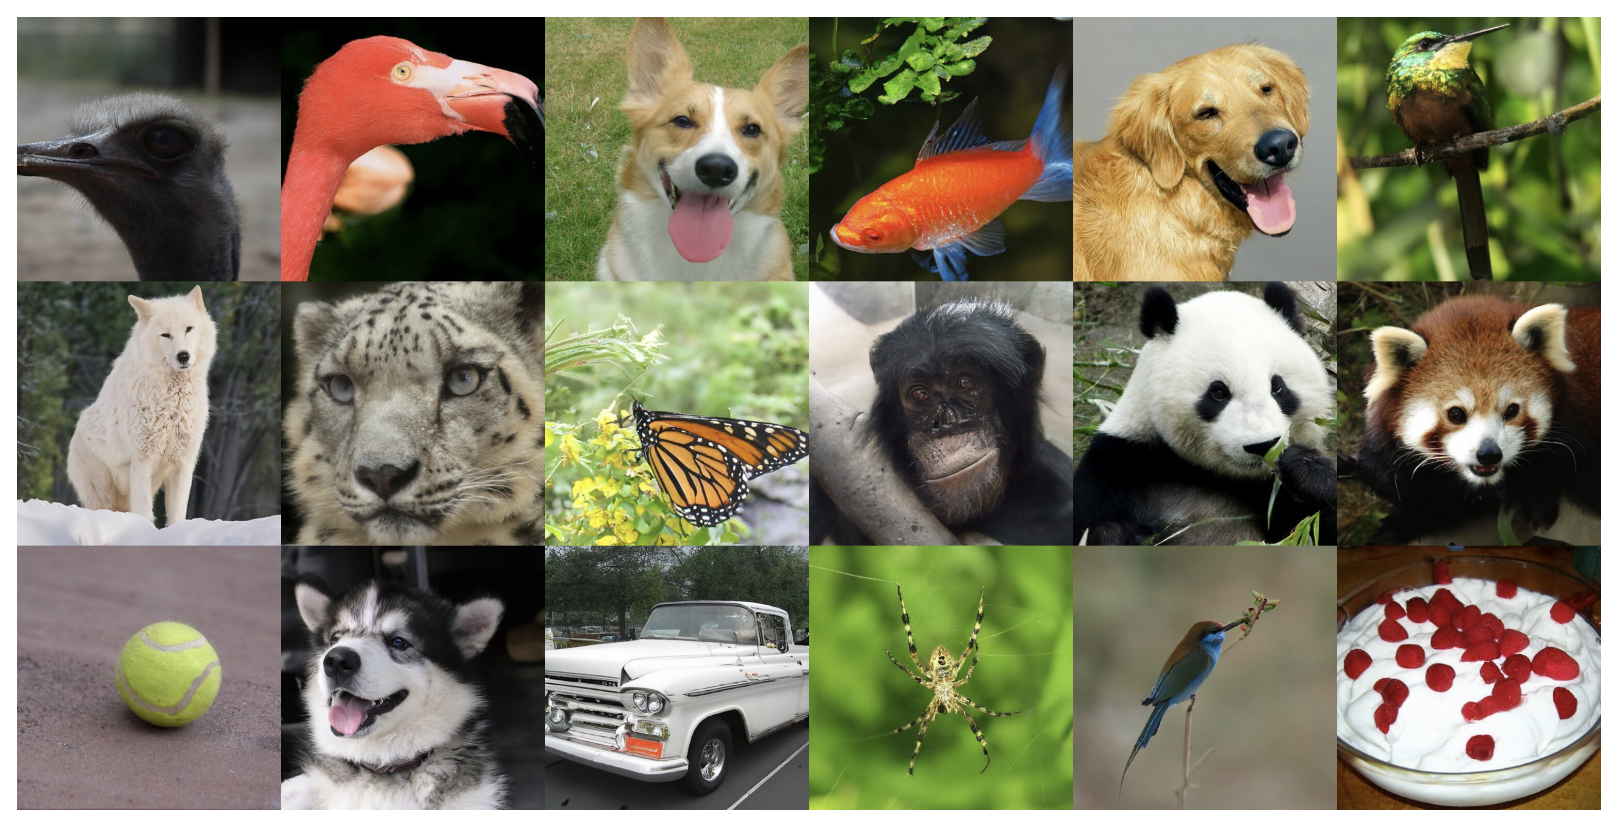
\includegraphics[width = 6in]{\images/DiffGAN}}

\slide{Conditional Diffusion Models}

We assume training data consisting of $(x,y)$ pairs and we want to generate from the distribution $P(y|x)$.  For example class-conditional image generation.

\vfill
Previous approaches, such as StyleGAN, have trained a model (a GAN) for each class.

\vfill
Here we will train a single model which takes the class label as input.

\slide{Conditional Diffusion Models}

An obvious approach is to pass the conditioning information $x$ to the image generator.

\vfill
Unfortunately this natural approach to conditioning generates poor images.

\vfill
It remains true that generating high quality images requires ``guidance''.

\vfill
There are two forms of guidance --- classifier guidance and self-guidance.

\slide{Classifier Guidance}
We assume a distribution on pairs $(x,y)$.

\vfill
We also assume {\bf a classifier} $P(x|y)$.  For example $x$ might be the ImageNET label for image $y$.

\vfill
We use $p(y|x) \propto P(y)P(x|y)$.

\vfill
We will generate an image by using $P(x|y)$ to ``guide'' generation from the unconditional model $\epsilon(z_\ell,\ell)$.

\begin{eqnarray*}
z(t - \Delta t) & = & z(t) + \eta\left(\nabla_z\ln P_t(z) +  s \nabla_z\;\ln P(x|z)\right)
\end{eqnarray*}

\vfill
Here $s$ is called the scale of the guidance.

\slide{Classifier Guidance}

\begin{eqnarray*}
z(t - \Delta t) & = & z(t) + \eta\left(\nabla_z\ln P_t(z) + s \nabla_z\;\ln P(x|z)\right)
\end{eqnarray*}

\vfill
\begin{eqnarray*}
{\color{red} \nabla_z \ln P_t(z)}&  {\color{red}  =} & {\color{red}\frac{E[y|t,z]-z}{t}}
\end{eqnarray*}


\vfill
Empirically it was found that $s > 1$ is needed to get good class-specificity of the generated image.

\vfill
However, increasing $s$ decreases diversity so we have a diversity/quality trade off.

\slide{Other Improvements}

Various architectural choices in the U-Net were optimized.

\vfill
These improvements are used in DALLE-2.

\slidetwo{Classifier-Free Diffusion Guidance}
{Ho and Salimans, (Google Brain, December 2021)}

Classification diffusion guidance uses a classification model $P(x|y)$.

\vfill
This paper introduces ``classifier-free'' diffusion guidance.

\vfill
Classifier-free diffusion guidance is used in DALLE-2.

\slide{Classifier-Free Diffusion Guidance}

5\% of the time we set $x = \emptyset$ where $\emptyset$ is a fixed value unrelated to the image.

\vfill
The prior then uses

\vfill
\begin{eqnarray*}
z(t - \Delta t) & = & z(t) + \eta\left(s\nabla_z\ln P_t(z|x) - (s-1) \nabla_z\;\ln P(z|\emptyset)\right)
\end{eqnarray*}

\slidetwo{Image Super-Resolution via Iterative Refinement}{Saharia, Ho et al., April 2021}

They construct a super-resolution diffusion model as conditional model for pairs for pairs $(x,y)$ with $x$ is a downsampling of $y$.

\vfill
\centerline{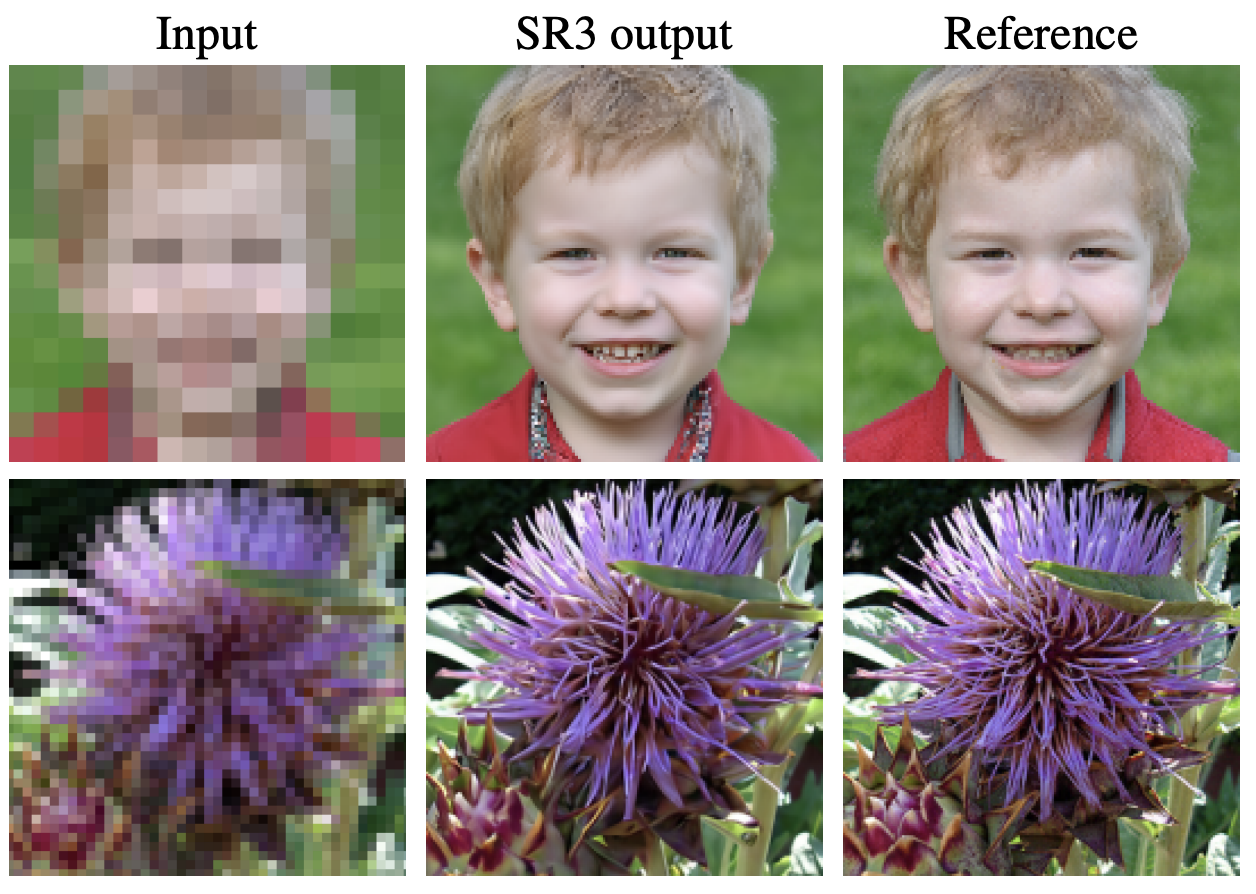
\includegraphics[width = 4 in]{\images/DiffUp1}}

\slidetwo{Cascaded Diffusion Models ...}{Ho, Saharia et al, May 2021}

A series of super-resolution diffusion models each conditioned on a class label.

\centerline{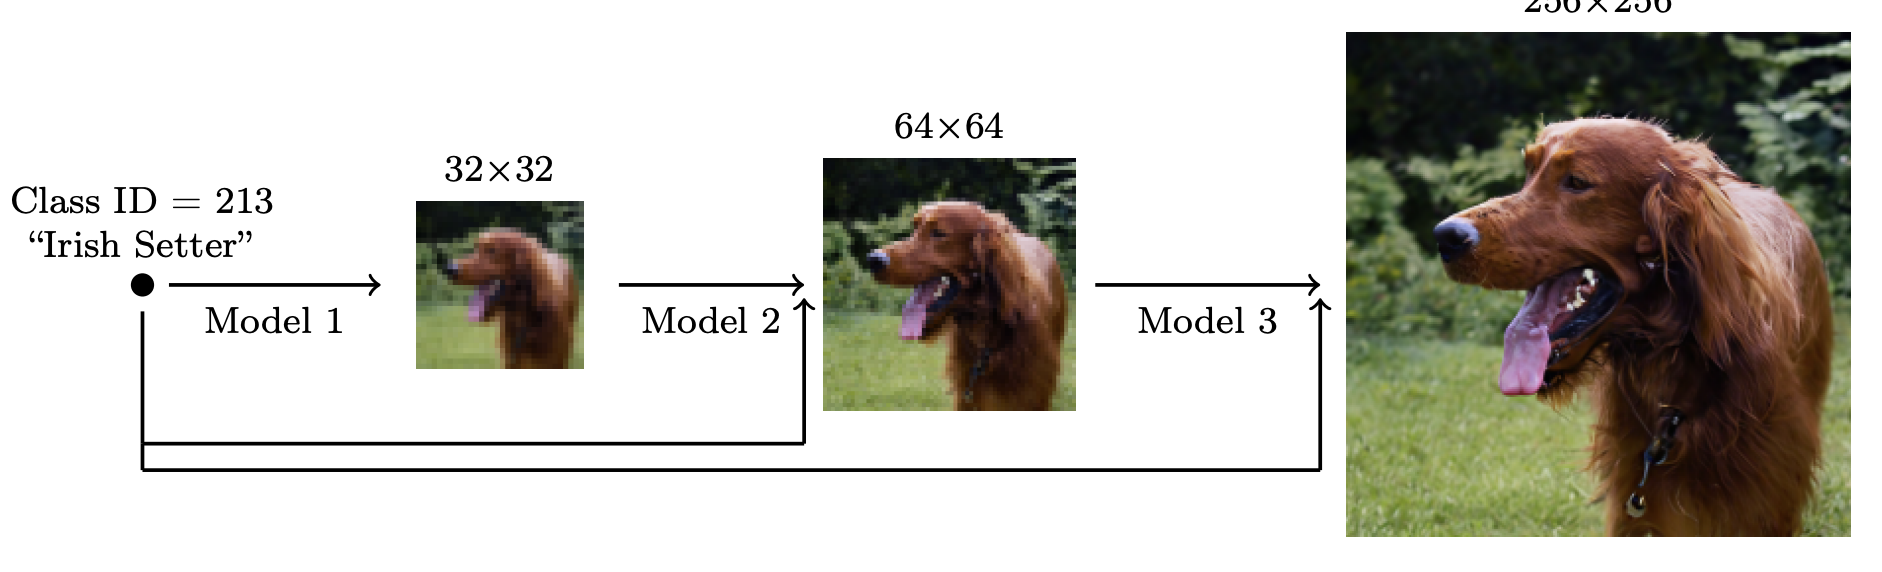
\includegraphics[width = 8 in]{\images/DiffUp2}}

\vfill
This architecture is used in DALLE-2.

\slide{CLIP Does Contrastive Coding}

\centerline{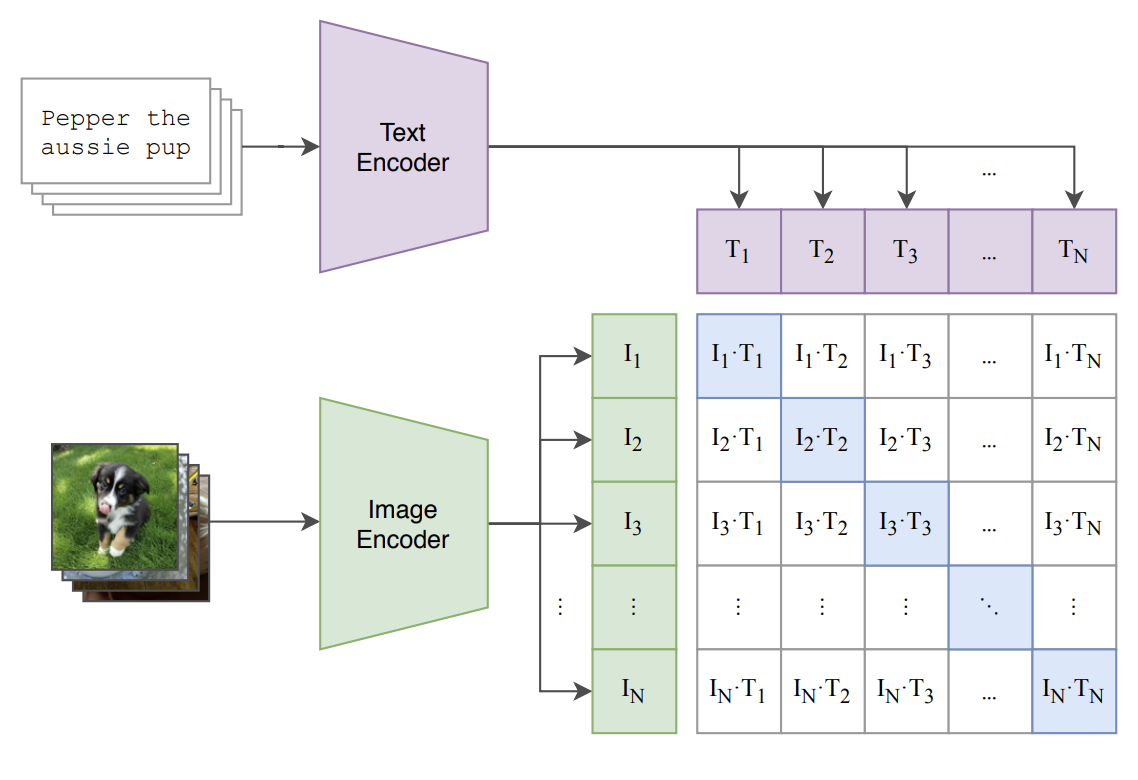
\includegraphics[height= 4in]{\images/CLIPTraining}}

\vfill
CLIP is used in DALLE-2 and in DALLE-2's predicessor GLIDE.

\slidetwo{GLIDE: Towards Photorealistic Image Generation ...}
         {Nichol, Dhariwal, Ramesh, et al., December 2021}

GLIDE compares two forms of diffusion guidance.

\vfill
\begin{itemize}
\item[(a)] Classifier-free guidance based on comparing conditioned and unconditioned decoding directions.

\vfill
\item[(b)] Classifer guidance based on CLIP.
\end{itemize}

\slide{Classifier-free (self-guided) GLIDE}

\vfill
Classifier-free GLIDE does not use CLIP.

\vfill
The classifier-free guidance differs from the original version in that here we are conditioning on text
rather than as Imagenet labels.

\vfill
The text is transformed to a feature vector by a transformer before being fed to the prior.

\slide{CLIP-guided GLIDE}

Let $C_I(y)$ be the CLIP vector for image $y$ and let $C_T(x)$ be the CLIP vector for text $x$.

\vfill
CLIP-based Glide approximates uses

\vfill
$$\ln P(z|x) \approx C_T(x)^\top C_I(z)$$

\vfill
CLIP is re-trained to handle noised images.

\slide{Upsamling}

Both GLIDE versions use diffusion upsampling to go from $64 \times 64$ to $256 \times 256$.

\vfill
The GLIDE paper concludes that the classifer-free model taking raw text as input is superior to the CLIP-guided model.

\slidetwo{DALL$\cdot$E-2}{Ramesh, Nichol, Dhariwal, et al., March 2022}

\centerline{\hfill 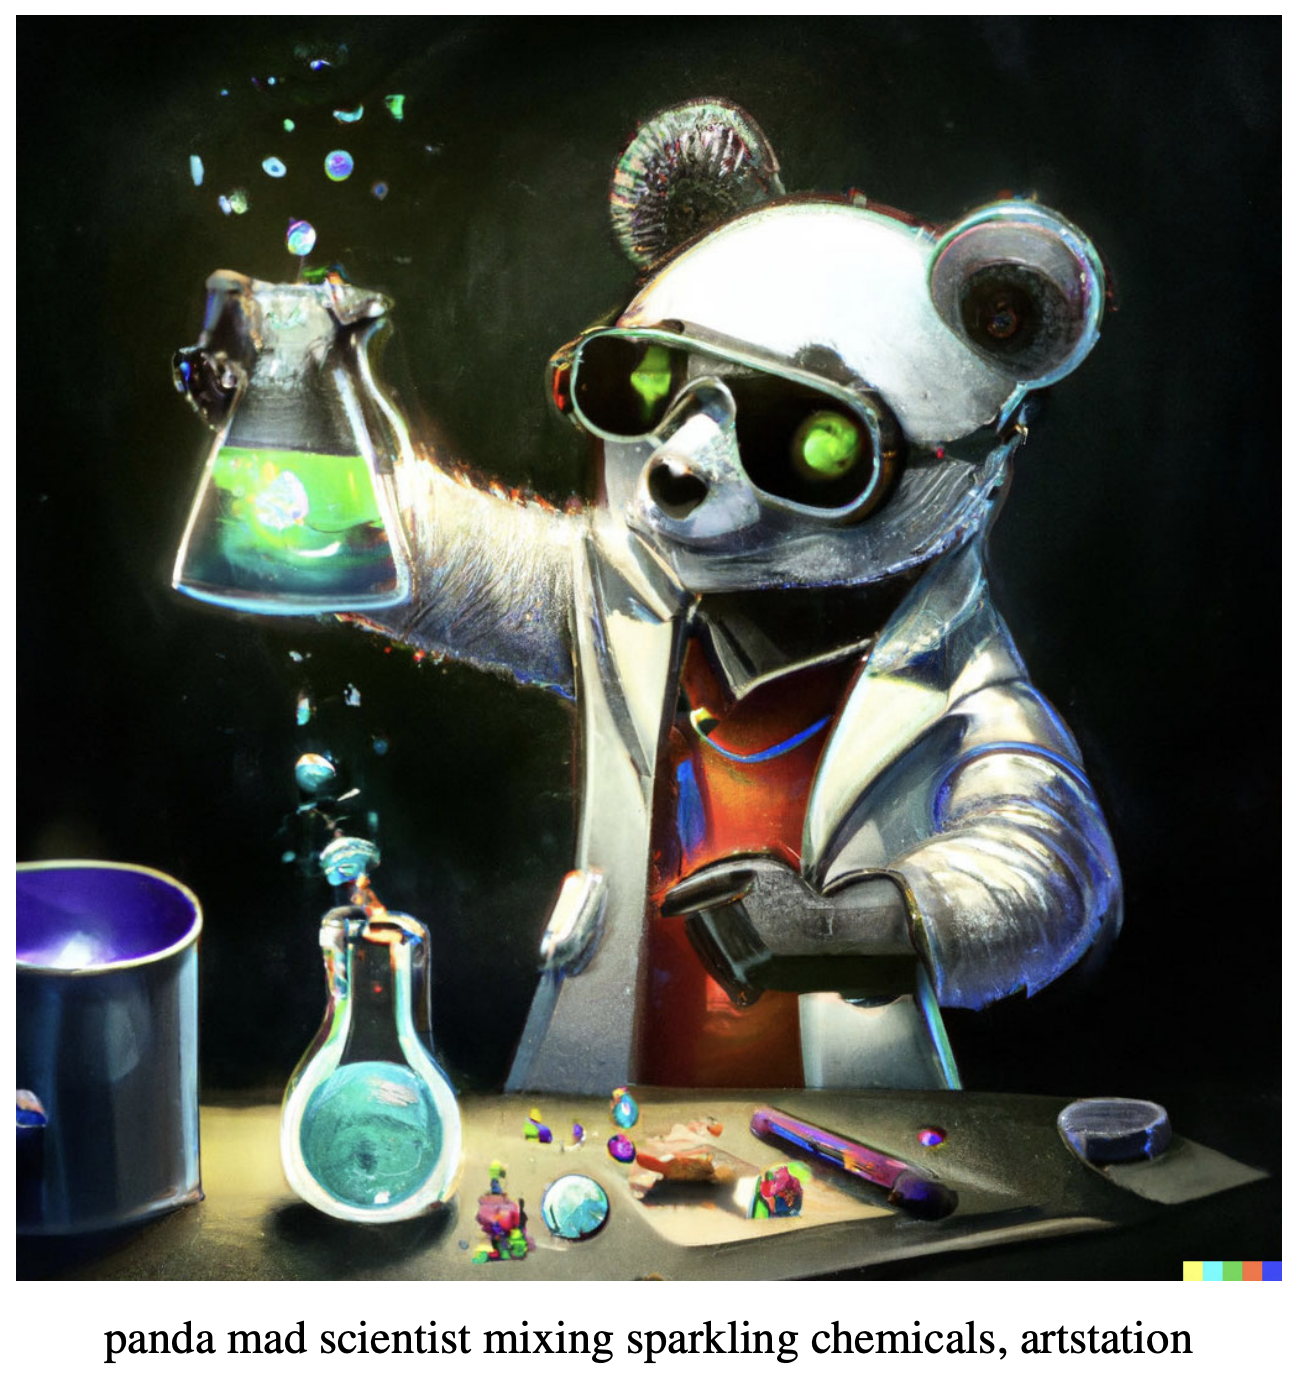
\includegraphics[width = 3.5 in]{\images/DALLEpanda} \hfill \includegraphics[width = 3in]{\images/DALLE2}}

CLIP-guided DALLE-2 is similar in quality to self-guided GLIDE but is more diverse.

\slide{DALL$\cdot$E-2}

\vfill
\centerline{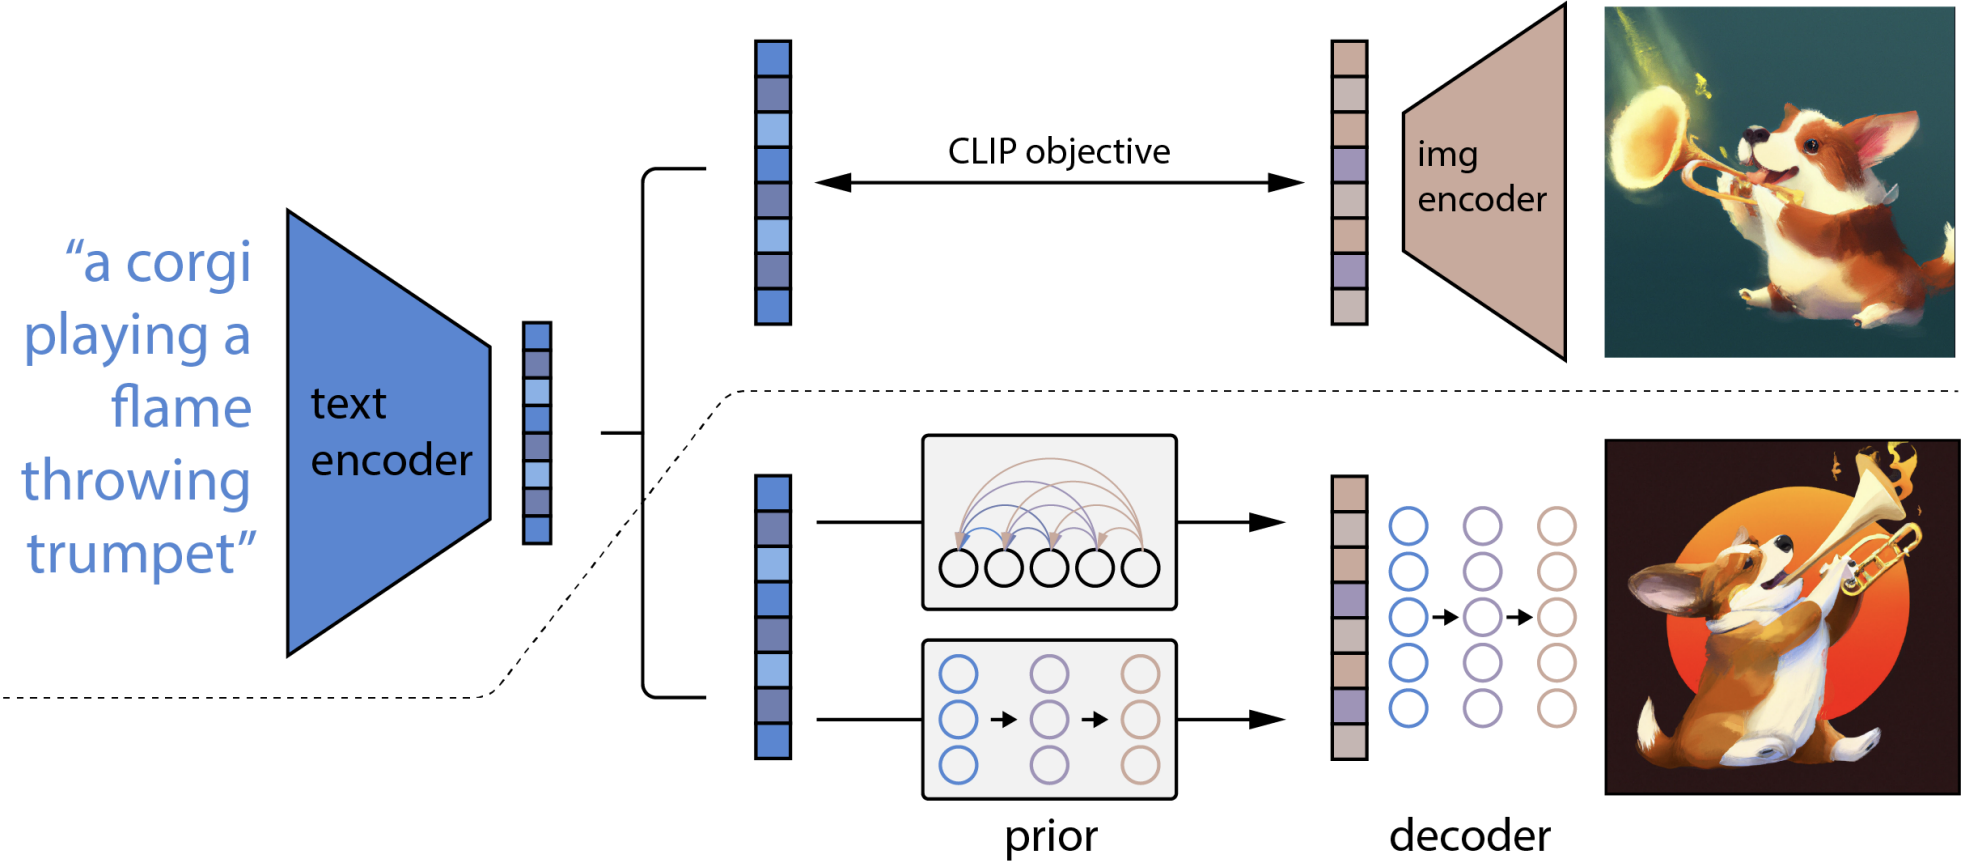
\includegraphics[width = 8in]{\images/DALLE2a}}

This figure is misleaning.  The lines in the figure do not correspond to the actual data paths of DALLE-2.

\slide{A Conditional Image Auto-Encoder}

\centerline{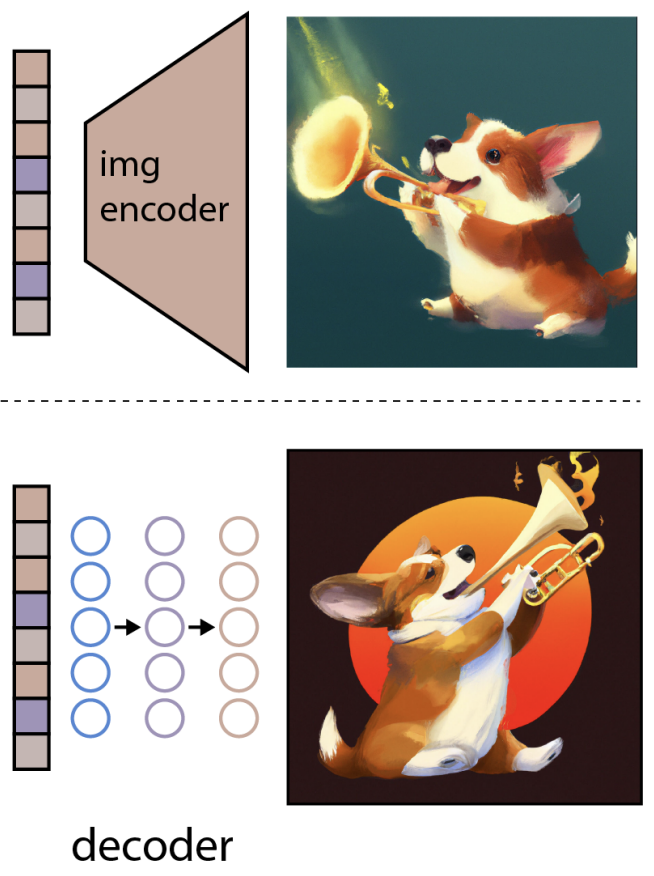
\includegraphics[height = 2.5in]{\images/DiffDALLE}}

\vfill
Let $C_I(y)$ denote the CLIP embedding of image $y$.

\vfill
$C_I(y)$ is taken to be the encoder of a VAE for $y$ given $x$.

\vfill
$P(C_I(y)|x)$ is the optimal prior for this auto-encoder.

\vfill
$P(y|C_I(y),x)$ is the optimal decoder.

\vfill
In DALLE-2 the prior and the generator both see the text $x$.

\slide{END}
}
\end{document}


